%%% File encoding is utf8
%%% You can use special characters just like ä,ü and ñ

\chapter{Formatierung und Umgang mit der Vorlage}
In diesem Kapitel wird die Handhabung mit dem Template vorgestellt und anhand verschiedener Beispiele gezeigt. Die Struktur des Dokuments soll simpel gehalten werden und basiert auf einer einfachen Ordnerstruktur. Diese ist wichtig, um auf die verschiedenen Dateien über das MainFile zugreifen zu können. Daher sollte die Ordnerstruktur unbedingt beibehalten werden.

\section{Preambles}
Die Preambles definieren die Formatierung (Schriftgröße, Seitenzahlen, Farben, etc.) des Dokuments und sollten \textbf{nicht} bearbeitet werden! Nur die Datei \textbf{PDF-Related} kann bearbeitet und die entsprechenden "Felder" ausgefüllt werden.

\section{Kapitel}
Jedes Oberkapitel hat seine eigene .tex Datei. Diese Dateien liegen in dem Ordner für Kapitel. Möchte man ein neues Kapitel erstellen, so legt man einfach eine neue Datei an und legt sie in diesem Ordner ab. Das Kapitel muss dann über das MainFile (siehe \ref{cha:mainFile}) in das Dokument eingebunden werden. Verschiedene Kapitel lassen sich auch, ähnlich zu einem Wiki-Artikel, untereinander verlinken. Dazu vergibt man dem jeweiligen Kapitel ein Label und ein Kürzel, über welches das jeweilige Kapitel angesprochen werden kann.

\section{MainFile}\label{cha:mainFile}
Im MainFile werden die verschiedenen Kapitel zu einem Dokument zusammengefügt. Hier werden keine Texte geschrieben, sondern nur die Dateien aus den entsprechenden Ordnern aufgerufen (\emph{siehe Abbildung}). Bearbeitet wird das MainFile erst ab dem Tag \textbf{begin document}. Die input-Befehle binden die Preambles in das Dokument ein.

\begin{figure}[H]
    \centering
    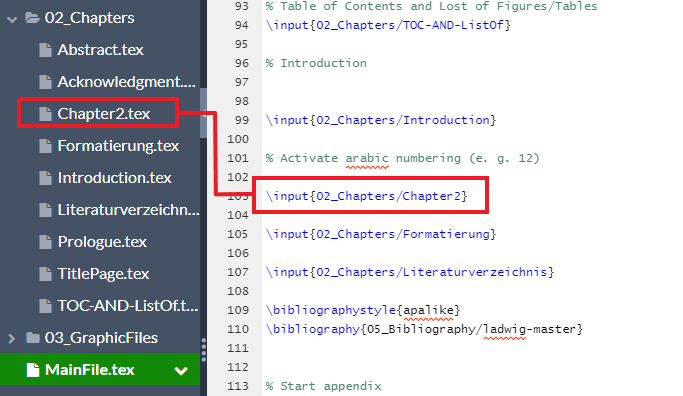
\includegraphics[width=\textwidth]{03_GraphicFiles/MainFile.png}
    \caption{Code-Snippet MainFile (Overleaf)}
    \label{fig:mainFile}
\end{figure}

\section{Abbildungen und Tabellen}
In diesem Abschnitt wird gezeigt, wie Abbildungen und Tabellen in das Dokument eingebunden werden. Das Abbildungs- und Tabellenverzeichnis wird automatisch aktualisiert sobald man eine Abbildung oder Tabelle korrekt einbindet und die PDF-Datei kompiliert.

\subsection{Abbildungen} \label{cha:figures}
Für Abbildungen wird ebenfalls ein eigener Ordner angelegt, über den die Dateien aufgerufen werden können.

\begin{figure}[H]
    \centering
    \includegraphics[width=\textwidth]{03_GraphicFiles/BilderEinfügen.png}
    \caption{Abbildungen korrekt einfügen}
    \label{fig:picture}
\end{figure}

Das \textbf{[H]}, in der Abbildung gelb markiert, sorgt dafür, dass das jeweilige Bild genau an der Stelle im Dokument eingefügt wird, an der sich das Bild auch im Code befindet. Ansonsten kann es passieren, dass die Bilder nicht an der richtigen Stelle im Dokument, eventuell sogar in einem anderen Kapitel, abgebildet werden.

\newpage
\subsection{Tabellen und Diagramme}
Tabellen lassen sich einfach erstellen, auch das Layout der Tabellen lässt sich schnell ändern.

\begin{table}[H]
	\centering
	\begin{tabular}{|| c | c | c | c | c | c ||}
	    \hline
		Spalte & Spalte & Spalte & Spalte & Spalte & Spalte \\ [0.5ex]
		\hline\hline
		Inhalt & Inhalt & Inhalt & Inhalt & Inhalt & Inhalt \\
		Zeile & Zeile & Zeile & Zeile & Zeile & Zeile \\
		Inhalt & Inhalt & Inhalt & Inhalt & Inhalt & Inhalt \\
		Zeile & Zeile & Zeile & Zeile & Zeile & Zeile \\
		\hline
	\end{tabular}
	\caption{Eine Tabelle erstellen}
	\label{tab:newTable}
\end{table}

\begin{figure}[H]
    \centering
    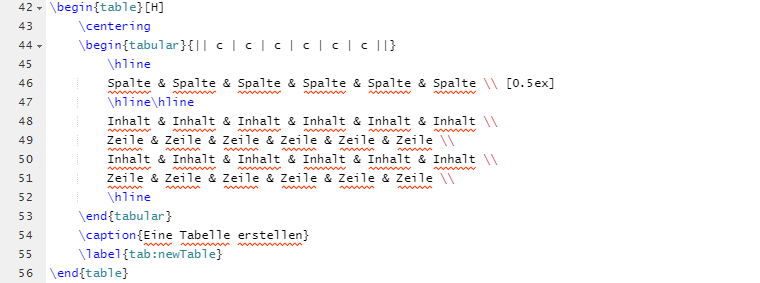
\includegraphics[width=\textwidth]{03_GraphicFiles/TabellenErstellen.PNG}
    \caption{Code-Snippet für Tabellen}
    \label{fig:createTable}
\end{figure}

Es lassen sich auch vorgefertigte Diagramme über LaTex erstellen und verändern. Verschiedene Arten von Diagrammen können mit dem \emph{smartdiagram-package} einfach und schnell generiert werden. Das Package stellt verschiedene Arten von Diagrammen bereit. Möchte man diese nutzen, so sollte man sich auf der entsprechenden Internetseite informieren. 

Hier zwei Beispiel-Diagramme:
\begin{figure}[H]
    \centering
    \smartdiagram[flow diagram:horizontal]{Schritt 1, Schritt 2, Schritt 3, Schritt 4, Schritt 5}
    \caption{Ein Flussdiagramm mit schönen Farben}
    \label{fig:flowdiagram}
\end{figure}

Die Diagramme werden erstellt wie Abbildungen (siehe \ref{cha:figures}). Anstatt \emph{includegraphics} wird bei Diagrammen einfach \emph{smartdiagram} aufgerufen. In den eckigen Klammern wird dann die Art des Diagramms definiert und in den geschweiften Klammern der Inhalt (siehe \ref{fig:diagrams}). Die Diagramme werden so auch im Abbildungsverzeichnis gelistet und können mit einer passenden Beschreibung versehen werden.

\begin{figure}
    \centering
    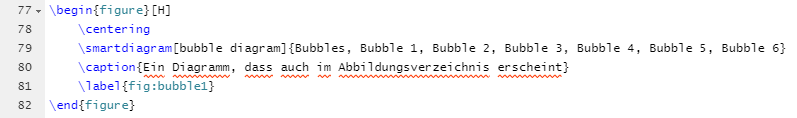
\includegraphics[width=\textwidth]{03_GraphicFiles/smartdiagram.PNG}
    \caption{How to diagram}
    \label{fig:diagrams}
\end{figure}

\begin{figure}[H]
    \centering
    \smartdiagram[bubble diagram]{Bubbles, Bubble 1, Bubble 2, Bubble 3, Bubble 4, Bubble 5, Bubble 6}
    \caption{Ein Diagramm, welches auch im Abbildungsverzeichnis gelistet wird}
    \label{fig:bubble1}
\end{figure}

\section{Literaturverzeichnis}
Für das Literaturverzeichnis ist es empfehlenswert ein Programm, beispielsweise Citavi, zu nutzen. Es gibt einige Programme, die sich problemlos in Verbindung mit LaTex nutzen lassen können. Über Citavi, beispielsweise, lässt sich direkt eine BibTex-Datei erstellen, die sich einfach in das Dokument einbinden lässt. \emph{Beispiel-Literatur für Literaturverzeichnis -} \cite{Butterworth1992}.
\emph{Beispiel-Literatur für Literaturverzeichnis -} \cite{Clark1976}
Für den Umgang mit Litertaturmanagement-Programmen und LaTex gibt es zahlreiche Tutorials, beispielsweise für  \href{https://www.youtube.com/watch?v=GmyCcvXrSDI}{Umgang mit LaTex und Citavi}




